%% nonmortal -- holes of the two-word problem with self events that are not
%% mortal: the continuation identity, the decomposition at the first rejected
%% cut, kinds of state, the breaker, lassos, short pre-holes, aperiodic
%% lassos, the pump for periodic lassos, and the three-case theorem.
%% Full proofs are in appendix-nonmortal.tex.

\section{Non-Mortal Holes}\label{sec:nm}

Let $I$ be an instance of the two-word hole problem with self events
(\cref{def:ex-ss2self}) that satisfies condition (FH) (\cref{def:ex-fh}). This section shows that if
$I$ has a hole, then it has a hole whose length is polynomial in the sizes of
its four automata, or it has a \emph{mortal hole}: a hole $(u,t)$ whose spine
ends in a state without infinite safe continuations and whose target ends
fewer than $N_A$ letters after its first rejected cut
(\cref{thm:nm-three-cases}). Mortal holes are treated in \cref{sec:mo}.

The argument starts from a simple observation. Cutting a hole $(u,t)$ at the
first rejected cut $J(t)$ of its target splits off the \emph{continuation}
$\theta=\wsuf t{J(t)}$. Condition (FH) places every target head before $J(t)$,
so $\theta$ is a common suffix of both words, and what remains is a shorter
pair $(u_0,t_0)$ with $u=u_0\theta$ and $t=t_0\theta$, a \emph{pre-hole}
(\cref{lem:nm-decomposition} and \cref{fig:nm-prehole}). Appending the same
word to both words creates no new events and no new self events, and it keeps
an existing one exactly when it continues the overhang of that event
periodically (\cref{lem:nm-continuation}). The question is therefore whether
a single continuation that keeps the spine automaton out of $\Bad$ can break
every pending obligation of a pre-hole: its events, which are never aligned,
and the self events of its target. The answer depends on the state
$q=A(u_0)$ at the end of the spine of the pre-hole.
\begin{itemize}[leftmargin=*]
\item If a cycle that offers a choice of two letters is reachable from $q$,
  a breaking continuation of length at most $\max(\len{u_0},\len{t_0})+3N_A$
  always exists (\cref{lem:nm-breaker}).
\item If every reachable cycle is forced, then the long continuations follow
  finitely many ultimately periodic words, the \emph{lassos} of $q$
  (\cref{lem:nm-thin}). A lasso that is not purely periodic breaks every
  obligation (\cref{lem:nm-aperiodic}). A purely periodic lasso may let
  obligations survive, and then the pre-hole itself has to be shortened. The
  \emph{pump} (\cref{thm:nm-pump}) deletes factors of the two words while
  keeping the endpoint $q$ and the absence of surviving obligations, down to a
  length polynomial in the sizes of the automata.
\item In the remaining cases the continuation reaches a state without
  infinite safe continuations within fewer than $N_A$ letters, and the hole is
  mortal.
\end{itemize}

\paragraph{Conventions}
We use the instance, safety, comparison, event, and forced-head conventions of
\cref{def:ex-ss2self,def:ex-events,def:ex-fh}. For an automaton $M$, let
$M(r,w)$ denote its state after reading $w$ from $r$, and let
$M_s(w)=M(0,\wpre ws)$ be its state at the cut $s$ of $w$. We abbreviate the
state counts as
\[
 a=N_A,\qquad b=N_B,\qquad a'=N_{A'},\qquad b'=N_{B'};
\]
all four are at least $1$.

An \emph{infinite word} $\xi'=\xi'[0]\xi'[1]\cdots$ over $\Sigma$ has prefixes
$\wpre{\xi'}k$ and suffixes $\wsuf{\xi'}k$ as for finite words, and $v\xi'$ is the
infinite word that starts with the finite word $v$. A number $\varpi\ge1$ is a
\emph{period} of $\xi'$ if $\xi'[i+\varpi]=\xi'[i]$ for all $i\ge0$; $\xi'$ is \emph{purely
periodic} if it has a period, and its \emph{least period} is then the least of
its periods. For a nonempty finite word $o$, $o^\omega=ooo\cdots$ is the
infinite word with period $\len o$ that begins with $o$; a finite word is a
prefix of $o^\omega$ exactly when it is a prefix of some $o^k$, in agreement
with the notation $\theta\pre o^\omega$ of \cref{sec:bg-words}. Holes are
written $(u,t)$, pre-holes $(u_0,t_0)$, continuations $\theta$, and infinite
words $\xi$.

\subsection{The Continuation Identity}\label{sec:nm-continuation}

For a cross comparison $(s,e)$ of $(u,t)$ and a word $\theta$, we say that
$\theta$ \emph{keeps} $(s,e)$ if $\wsuf te\,\theta\pre\wsuf us\,\theta$, and
that $\theta$ \emph{breaks} it otherwise; for a self comparison $(i,j)$ of $t$,
$\theta$ keeps it if $\wsuf tj\,\theta\pre\wsuf ti\,\theta$. Non-aligned cross
comparisons can be unboundedly many: if $u=\ell^k$ and $t=\ell^m$ for a letter
$\ell$, every pair of cuts with a nonnegative offset is one. We therefore do
not count them but control them through common continuations.

\begin{lemma}[Continuation identity]\label{lem:nm-continuation}
Let $u$, $t$ and $\theta$ be words such that $J(t)$ is defined.
\begin{enumerate}[label=(\alph*)]
\item $J(t\theta)=J(t)$, and each of the four automata has the same state at
every cut $s\le\len u$ of $u\theta$ as at the cut $s$ of $u$, and at every cut
$e\le\len t$ of $t\theta$ as at the cut $e$ of $t$.
\item Let $s\le\len{u\theta}$ and $e\le J(t)$. Then $(s,e)$ is a cross
comparison of $(u\theta,t\theta)$ if and only if $s\le\len u$, $(s,e)$ is a
cross comparison of $(u,t)$, and $\theta$ keeps it. Likewise, for
$i<j\le J(t)$, the pair $(i,j)$ is a self comparison of $t\theta$ if and only
if it is a self comparison of $t$ and $\theta$ keeps it.
\item A word $\theta$ keeps a cross or self comparison with overhang $o$ if and
only if $\theta\pre o\theta$. If $o\ne\eps$, this holds if and only if
$\theta\pre o^\omega$. Every word keeps every aligned cross comparison.
\end{enumerate}
\end{lemma}

In words: a common continuation creates no new comparison among the cuts up to
$J(t)$, and it keeps an existing one exactly when it continues the overhang
periodically. The proof is in \cref{app:nm-continuation}. We use the lemma
through the following \emph{continuation facts}, which hold for all words $u$
and $t$ with $J(t)$ defined and every word $\theta$:
\begin{enumerate}[label=(K\arabic*)]
\item the events of $(u\theta,t\theta)$ are exactly the events of $(u,t)$ that
$\theta$ keeps, and the self events of $t\theta$ are exactly the self events of
$t$ that $\theta$ keeps;
\item every word keeps every aligned cross comparison, so aligned events can
never be removed;
\item if $\theta$ breaks a cross or self comparison, so does every word with
prefix $\theta$;
\item every head event of $(u,t)$ is a head event of $(u\theta,t\theta)$;
\item if $u$ is safe, then $u\theta$ is safe if and only if $\theta$ is safe
from $A(u)$.
\end{enumerate}
A non-aligned event or a self event with overhang $o$ is thus a periodicity
obligation: a continuation removes it exactly when it departs from $o^\omega$.

\subsection{Pre-Holes and the Decomposition at the First Rejected Cut}\label{sec:nm-prehole}

\begin{definition}[Pre-hole]\label{def:nm-prehole}
A \emph{pre-hole} of $I$ is a pair $(u_0,t_0)$ such that $u_0$ is safe,
$J(t_0)=\len{t_0}$, $(u_0,t_0)$ has a head event, and $(u_0,t_0)$ has no aligned
event. Its \emph{obligations} are its events and the self events of $t_0$. A
word $\theta$ \emph{completes} $(u_0,t_0)$ if $\theta$ is safe from $A(u_0)$ and
breaks every obligation of $(u_0,t_0)$.
\end{definition}

No obligation of a pre-hole is aligned, so every obligation has a nonempty
overhang. The overhang of an event has length at most $\len{u_0}$ and that of a
self event at most $\len{t_0}$, so every obligation has an overhang of length at
most
\[
 W=\max(\len{u_0},\len{t_0}).
\]
A pre-hole without obligations is a hole, completed by the empty word.

\begin{figure}[t]
\centering
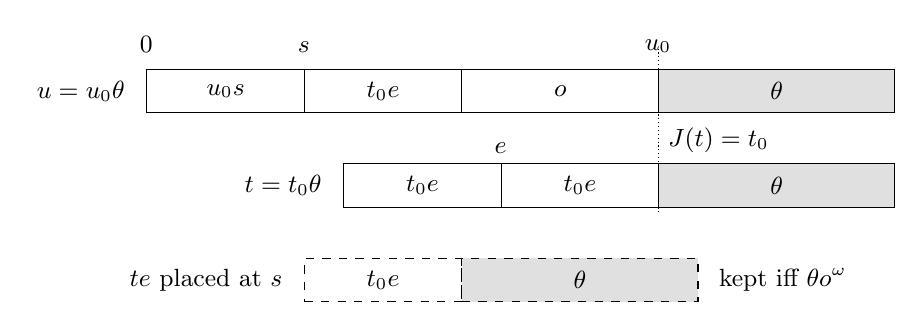
\begin{tikzpicture}[x=1cm,y=1.2cm,font=\small,
  box/.style={draw,minimum height=0.55cm,inner sep=0pt},
  cont/.style={box,fill=black!12},
  shifted/.style={box,dashed}]
  % spine u = u_0 theta
  \node[box,minimum width=2.0cm,anchor=west] at (0,2) {$\wpre{u_0}{s}$};
  \node[box,minimum width=2.0cm,anchor=west] at (2,2) {$\wsuf{t_0}{e}$};
  \node[box,minimum width=2.5cm,anchor=west] at (4,2) {$o$};
  \node[cont,minimum width=3.0cm,anchor=west] at (6.5,2) {$\theta$};
  \node[anchor=east] at (-0.15,2) {$u=u_0\theta$};
  % target t = t_0 theta
  \node[box,minimum width=2.0cm,anchor=west] at (2.5,1) {$\wpre{t_0}{e}$};
  \node[box,minimum width=2.0cm,anchor=west] at (4.5,1) {$\wsuf{t_0}{e}$};
  \node[cont,minimum width=3.0cm,anchor=west] at (6.5,1) {$\theta$};
  \node[anchor=east] at (2.35,1) {$t=t_0\theta$};
  % the target suffix t[e:] = t_0[e:] theta placed at the cut s of u
  \node[shifted,minimum width=2.0cm,anchor=west] at (2,0) {$\wsuf{t_0}{e}$};
  \node[shifted,fill=black!12,minimum width=3.0cm,anchor=west] at (4,0) {$\theta$};
  \node[anchor=east] at (1.85,0) {$\wsuf te$ placed at $s$};
  \node[anchor=west] at (7.15,0) {kept iff $\theta\pre o^\omega$};
  % cuts
  \draw[densely dotted] (6.5,2.45) -- (6.5,0.72);
  \node[above] at (0,2.3) {$0$};
  \node[above] at (2,2.3) {$s$};
  \node[above] at (6.5,2.3) {$\len{u_0}$};
  \node[above,inner sep=2pt] at (4.5,1.28) {$e$};
  \node[above right,inner sep=2pt] at (6.55,1.28) {$J(t)=\len{t_0}$};
\end{tikzpicture}
\Description{Three rows of boxes. The top row is the spine, divided into
the prefix of the pre-hole spine before the cut s, a copy of the target
suffix from cut e, the overhang o, and the shaded continuation theta. The
middle row is the target, right-aligned with the spine, divided into the
target prefix before e, the target suffix from e, and the shaded
continuation theta; a dotted line marks the first rejected cut. The bottom
row places the target suffix and theta at the cut s of the spine, so that
theta lies below the overhang.}
\caption{A hole $(u,t)=(u_0\theta,t_0\theta)$ cut at the first rejected cut
$J(t)=\len{t_0}$ of its target (\cref{lem:nm-decomposition}); the continuation
$\theta$ is shaded. An event $(s,e)$ of the pre-hole $(u_0,t_0)$ places
$\wsuf{t_0}e$ at the cut $s$ of $u_0$, followed by the overhang $o=o(s,e)$.
After $\theta$ is appended, $(s,e)$ is still a cross comparison if and only if
the shifted copy of $\theta$ (bottom row) agrees with $o\theta$, that is, if
and only if $\theta\pre o^\omega$ (\cref{lem:nm-continuation}). A self event
$(i,j)$ of $t_0$ behaves in the same way, with $t_0$ in the top row. A hole
requires $\theta$ to break every event and every self event.}
\label{fig:nm-prehole}
\end{figure}

\begin{lemma}[Decomposition at the first rejected cut]\label{lem:nm-decomposition}
If $(u_0,t_0)$ is a pre-hole and $\theta$ completes it, then
$(u_0\theta,t_0\theta)$ is a hole. Conversely, let $I$ satisfy \textup{(FH)} and
let $(u,t)$ be a hole. Then $\theta=\wsuf t{J(t)}$ is a suffix of $u$, and if
$u=u_0\theta$ and $t=t_0\theta$, then $(u_0,t_0)$ is a pre-hole and $\theta$
completes it.
\end{lemma}

In one direction, appending a completing word keeps the spine safe, keeps the
head event, and leaves no event and no self event, by (K5), (K4) and (K1). In
the other, (FH) places the target head of a head event before $J(t)$
(\cref{lem:ex-head-before-J}). Hence
$\theta$ is no longer than the common suffix and can be split off both words,
and (K1) and (K2) show that $\theta$ breaks every obligation of $(u_0,t_0)$ and
that $(u_0,t_0)$ has no aligned event. The proof is in
\cref{app:nm-continuation}. Condition (FH) cannot be dropped
(\cref{ex:nm-fh}).

\begin{example}[Shift closure: decomposition]\label{ex:nm-running}
In the instance $I_{y^1x^1}$ of \cref{ex:ex-running}, every target $t$ has
$J(t)=0$. So the hole $(01,1)$ splits as $\theta=\wsuf t0=1$ and
$(u_0,t_0)=(0,\eps)$. The pre-hole $(0,\eps)$ has the head event $(1,0)$,
and this aligned pair is not an event, because $A_1(0)=\{g^1\}$ misses
$P^{\varphi'_1}_{y^1}(\eps)=\{y^1,x^1\}$. Its only obligation is the event
$(0,0)$, with overhang $0$; the target $\eps$ has no self comparison. By
\cref{lem:nm-continuation}(c), a continuation keeps this obligation iff it is a
prefix of $0^\omega$. So the continuation $0$ keeps it, and indeed $(00,0)$
has the event $(0,0)$, while every continuation that contains the letter $1$
breaks it; the shortest one, $\theta=1$, gives back the hole $(01,1)$.
\end{example}

\subsection{Kinds of State}\label{sec:nm-kinds}

Let $\mathcal G_A$ be the \emph{safe graph} of $A$: its vertices are the safe
states of $A$, with an edge from $r$ to $A(r,\ell)$, labeled by the letter
$\ell$, whenever $A(r,\ell)$ is safe. The labels of the paths from $r$ are
exactly the words safe from $r$. A safe state is \emph{cyclic} if it lies on a
cycle of $\mathcal G_A$, and a letter $\ell$ is \emph{safe at} a safe state $r$
if $A(r,\ell)$ is safe.

\begin{definition}[Kinds of state]\label{def:nm-kinds}
A safe state $q$ of $A$ is
\begin{itemize}
\item \emph{mortal} if no infinite word is safe from $q$, equivalently, if no
cyclic state is reachable from $q$ in $\mathcal G_A$;
\item \emph{branching} if some cyclic state $r$ reachable from $q$ in
$\mathcal G_A$ has two distinct safe letters $\ell\ne\ell'$;
\item \emph{thin} if it is neither mortal nor branching.
\end{itemize}
\end{definition}

From a mortal state every safe run dies within $N_A$ letters. From a branching
state some reachable cycle offers a choice of letters, so a safe continuation
can depart from any given period. From a thin state infinite safe runs exist,
but once they reach a cycle they are forced, letter by letter. The two
descriptions of mortality agree because an infinite path in the finite graph
$\mathcal G_A$ repeats a vertex, and a reachable cyclic state can be visited
forever. A branching state reaches a cyclic state, so it is not mortal; the
three kinds are therefore pairwise disjoint, and every safe state has exactly
one of them. Each kind is decided by reachability in $\mathcal G_A$.

Branching asks only for two distinct safe letters at a reachable cyclic state;
the states they lead to may coincide, and the letter that leaves the cycle
need not admit any further safe continuation, since the breaker stops right
after it. Requiring all letters, or two specific letters, to be safe would
misclassify states over larger alphabets. For instance, for arity $n\le1$ no
state has two distinct safe letters, and for $n=0$ there are no letters at
all.

\subsection{The Breaker}\label{sec:nm-breaker}

\begin{lemma}[Breaker]\label{lem:nm-breaker}
Let $q$ be a branching state and $W\ge0$. There is a word $\theta$, safe from
$q$, with $\len\theta\le W+3N_A$, that is not a prefix of $o^\omega$ for any
word $o$ with $1\le\len o\le W$. In particular, every pre-hole $(u_0,t_0)$ with
$A(u_0)$ branching is completed by a word of length at most
$\max(\len{u_0},\len{t_0})+3N_A$.
\end{lemma}

The idea is to steer the spine into a cycle that offers a choice of letters, to
run around it for longer than any overhang, and then to leave it. The word
$\theta=\alpha\lambda^k\ell$ follows a shortest path $\alpha$ to a cyclic state
$r$ with two distinct safe letters, runs $k$ times around a shortest cycle
$\lambda$ through $r$, with $k\len\lambda\ge W+\len\lambda$, and leaves the
cycle by a safe letter $\ell\ne\lambda[0]$; one of the two safe letters at $r$
differs from $\lambda[0]$. If $\theta$ were a prefix of $o^\omega$, then over
the stretch $\lambda^k$, of length at least $\len o+\len\lambda$, it would have
both periods $\len o$ and $\len\lambda$, hence the period
$\gcd(\len o,\len\lambda)$ by the theorem of Fine and Wilf
\citep{FineWilf65}. So after $\lambda^k$ it would have to continue with
$\lambda[0]$, not with $\ell$. This uses only equality of letters and holds
over every alphabet. Every obligation of a pre-hole has a nonempty overhang of
length at most $W=\max(\len{u_0},\len{t_0})$, so $\theta$ breaks it by
\cref{lem:nm-continuation}(c). The proof is in \cref{app:nm-breaker}.

In \cref{ex:nm-running}, the spine state $A(0)=\{g^1\}$ lies on a loop at
which both letters are safe, so it is branching, and the breaker also
completes the pre-hole $(u_0,t_0)=(0,\eps)$. Here $W=1$, and the
construction may take the cyclic state $r=\{g^1\}$ itself, $\alpha=\eps$, the
cycle $\lambda=0$ and $k=2$; this gives $\theta=\alpha\lambda^k\ell=001$ with
the breaker letter $\ell=1$ and the hole $(0001,001)$, while the shortest
completion $\theta=1$ gives back $(01,1)$.

The bound uses $\max(\len{u_0},\len{t_0})$ because the overhang of a self
event of $t_0$ can be as long as $t_0$, which may be longer than $u_0$. The
maximum cannot be replaced by $\len{u_0}$, as the following example shows.

\begin{example}[Self events need the longer word]\label{ex:nm-max}
Let $\Sigma=\{0,1\}$ and $t_0=0001011100$. Let $A$ and $A'$ have a single state
$0$, with $\Bad=\varnothing$, so that $N_A=1$ and the state $0$ of $A$ is
branching, and let $\Guard=\varnothing$. Let $B$ and $B'$ both be the automaton
whose states are the prefixes of $t_0$, with start state $\eps$, and one sink;
it moves from $v$ to $v\ell$ while $v\ell$ is a prefix of $t_0$, and to the
sink otherwise. Let $\Rej=\{t_0\}$, let $\Head$ consist of the pair of the
state of $A'$ and the state $t_0$ of $B'$, and let $\GuardS$ consist of the
pairs $(\wpre{t_0}i,t_0)$ of states of $B$ with $0\le i\le7$. Condition (FH)
holds, since $t_0$ is the only word that leads $B'$ to the state $t_0$, and
its proper prefixes are not rejected. The pair $(\eps,t_0)$ is a pre-hole, and
its obligations are the self events $(i,10)$ with $0\le i\le7$, whose
overhangs are the suffixes $\wsuf{t_0}i$, of length at least $3$. The eight
factors $\wsub{t_0}i{i+3}$, $0\le i\le7$, are the eight words of length $3$
over $\Sigma$. So every word $\theta$ of length at most $3$ is a prefix of some
$\wsuf{t_0}i$ with $i\le7$ and keeps the self event $(i,10)$. Hence no word of
length at most $\len{u_0}+3N_A=3$ completes $(\eps,t_0)$, whereas
\cref{lem:nm-breaker} provides a completion of length at most
$\len{t_0}+3N_A=13$.
\end{example}

\subsection{Thin States and Lassos}\label{sec:nm-thin}

A \emph{lasso} of a safe state $q$ is an infinite word $\alpha\lambda^\omega$
with $\lambda\ne\eps$, $\len\alpha+\len\lambda\le N_A$, $\alpha\lambda$ safe
from $q$, and $A(q,\alpha\lambda)=A(q,\alpha)$. Every lasso of $q$ is safe from
$q$, and there are finitely many.

\begin{lemma}[Thin states]\label{lem:nm-thin}
Let $q$ be a safe state of $A$.
\begin{enumerate}[label=(\alph*)]
\item If $q$ is mortal, every word safe from $q$ has length less than $N_A$
and leads to a mortal state.
\item If $q$ is thin, every cyclic state reachable from $q$ has exactly one
safe letter, and the edge along it leads to a cyclic state.
\item If $q$ is thin, every infinite word safe from $q$ is a lasso of $q$, and
$q$ has at least one lasso.
\item If $q$ is thin, $\theta$ is safe from $q$, and $A(q,\theta)$ is mortal,
then $\len\theta<N_A$.
\end{enumerate}
\end{lemma}

Thus a thin region consists of finitely many lassos together with acyclic
paths into mortal states. Each part follows a safe run until it repeats a
state; the proof is in \cref{app:nm-breaker}.

\begin{definition}[Survival]\label{def:nm-survival}
A cross or self comparison \emph{survives} an infinite word $\xi$ if every
finite prefix of $\xi$ keeps it. An infinite word $\xi$ is
\emph{survivor-free} for a pre-hole $(u_0,t_0)$ if no obligation of
$(u_0,t_0)$ survives $\xi$.
\end{definition}

\begin{lemma}[Survival]\label{lem:nm-survival}
Let $u$ and $t$ be words and $\xi$ an infinite word.
\begin{enumerate}[label=(\alph*)]
\item A cross or self comparison with nonempty overhang $o$ survives $\xi$ if
and only if $\xi=o^\omega$. Every aligned cross comparison survives $\xi$.
\item Let $s\le\len u$ and $e\le\len t$ with $\len t-e\le\len u-s$. Then
$(s,e)$ is a cross comparison of $(u,t)$ that survives $\xi$ if and only if
$\wsuf us\,\xi=\wsuf te\,\xi$. Likewise, for $i<j\le\len t$, the pair $(i,j)$
is a self comparison of $t$ that survives $\xi$ if and only if
$\wsuf ti\,\xi=\wsuf tj\,\xi$.
\item Let $\xi=\alpha\lambda^\omega$ with $\lambda\ne\eps$. If a comparison
with nonempty overhang $o$ does not survive $\xi$, then the prefix of $\xi$ of
length $\len\alpha+\len\lambda+\len o-1$ breaks it.
\end{enumerate}
\end{lemma}

Part (a) is \cref{lem:nm-continuation}(c) applied to every prefix of $\xi$.
Part (b) turns survival into an equality of infinite words, which is the form
used by the pump; it holds because two finite words are prefixes of the same
infinite word exactly when the shorter is a prefix of the longer. Part (c)
compares two ultimately periodic words by the theorem of Fine and Wilf. The
proofs are in \cref{app:nm-survival}.

\begin{corollary}[Lasso completion]\label{cor:nm-lasso-completion}
Let $(u_0,t_0)$ be a pre-hole, and let $\xi$ be a lasso of $A(u_0)$ that is
survivor-free for $(u_0,t_0)$. Then the prefix of $\xi$ of length
$\max(\len{u_0},\len{t_0})+N_A-1$ completes $(u_0,t_0)$.
\end{corollary}

\begin{proof}
The prefix is safe from $A(u_0)$, since $\xi$ is. Write
$\xi=\alpha\lambda^\omega$ with $\len\alpha+\len\lambda\le N_A$. Each
obligation has a nonempty overhang $o$ with $\len o\le\max(\len{u_0},\len{t_0})$
and does not survive $\xi$. By \cref{lem:nm-survival}(c) the prefix of $\xi$ of
length $\len\alpha+\len\lambda+\len o-1\le\max(\len{u_0},\len{t_0})+N_A-1$
breaks it, and by (K3) so does the longer prefix.
\end{proof}

\subsection{Short Pre-Holes}\label{sec:nm-short}

Pre-holes form a recognizable set of pairs. A pre-hole asks for a safe spine,
a target rejected exactly at its end, and conditions on the aligned pairs of
cuts only, and the aligned pairs are the pairs at equal distance from the ends
within the longest common suffix. A finite graph that reads both words
forward, aligned at their right ends, can therefore track the four automata
and two bits: whether some aligned pair seen so far carries $\Head$, and
whether some carries $\Guard$. Both bits are reset whenever the two words
read different letters. Its paths spell exactly the pre-holes, and a shortest
path visits no node twice.

\begin{proposition}[Short pre-holes]\label{prop:nm-short-prehole}
Let $E$ be a set of safe states of $A$. If some pre-hole $(u_0,t_0)$ has
$A(u_0)\in E$, then some pre-hole $(u_1,t_1)$ has $A(u_1)\in E$ and
$\len{u_1},\len{t_1}<12aba'b'$. In particular, it is decidable whether a pre-hole
with $A(u_0)\in E$ exists.
\end{proposition}

The graph has the nodes $(r_A,r_B,r_{A'},r_{B'},h,g,\phi)$, with a state of
each automaton, two bits $h$ and $g$, and a phase $\phi\in\{0,1,2\}$ that
records whether only the spine, only the target, or both words are being read;
hence $12aba'b'$ nodes. The construction and its correctness are in
\cref{app:nm-graph}. The proposition does not preserve survivor-freeness for a
given lasso; it is used where every pre-hole with the given endpoint is good
enough, namely for branching endpoints and for lassos that are not purely
periodic.

\subsection{Aperiodic Lassos}\label{sec:nm-aperiodic}

\begin{lemma}[Aperiodic lassos]\label{lem:nm-aperiodic}
If an infinite word $\xi$ is not purely periodic, then no cross or self
comparison with a nonempty overhang survives $\xi$. In particular, $\xi$ is
survivor-free for every pre-hole.
\end{lemma}

\begin{proof}
By \cref{lem:nm-survival}(a), a comparison with nonempty overhang $o$ survives
$\xi$ only if $\xi=o^\omega$, which is purely periodic. Every obligation of a
pre-hole has a nonempty overhang.
\end{proof}

\subsection{The Pump}\label{sec:nm-pump}

The remaining non-mortal case is a pre-hole whose spine ends in a thin state
$q$ and a purely periodic lasso of $q$ that is survivor-free for it. Here
survivor-freeness depends on the pre-hole, and it can fail for short pre-holes
and hold for long ones, so \cref{prop:nm-short-prehole} does not apply. The
pump shortens the pre-hole directly, keeping its endpoint and its
survivor-freeness. Put
\[
 \Pcap(a,b,a',b')=2aba'b'+a^2a'+ab+aa'+bb' .
\]

\begin{theorem}[Pump]\label{thm:nm-pump}
Let $\xi$ be a purely periodic infinite word with least period $\varpi$, and let
$(u,t)$ be a pre-hole for which $\xi$ is survivor-free. Then there is a
pre-hole $(u',t')$ for which $\xi$ is survivor-free, with $A(u')=A(u)$ and
\[
 \len{u'},\len{t'}<2aba'b'+aa'\varpi+b\varpi+aa'+bb' .
\]
In particular, if $\varpi\le N_A$, then $\len{u'},\len{t'}<\Pcap(a,b,a',b')$.
\end{theorem}

The theorem uses no property of the state $A(u)$, and a lasso enters only
through the bound on its period: if a lasso $\xi=\alpha\lambda^\omega$ is purely
periodic, then its least period is at most $\len\lambda\le N_A$
(\cref{lem:nm-infinite}(b)), so the second bound applies. The proof rests on three
observations and a count; the details are in \cref{app:nm-pump}.

\emph{Survival as an equality of infinite words.} By
\cref{lem:nm-survival}(b), a pre-hole $(u,t)$ is survivor-free for $\xi$ if and
only if no pair of cuts $(s,e)$ with $\len t-e\le\len u-s$ and
$\wsuf us\,\xi=\wsuf te\,\xi$ carries $\Guard$, and no pair of cuts $i<j$ of $t$
with $\wsuf ti\,\xi=\wsuf tj\,\xi$ carries $\GuardS$; the aligned pairs are
among the former. Call such pairs \emph{$\xi$-matched}. The pump only has to
make sure that a deletion creates no new $\xi$-matched pair.

\emph{Rests and periodic ends.} Call a cut $s$ of a word $w$ \emph{periodic}
if $\wsuf ws\,\xi$ has period $\varpi$. The periodic cuts form an interval
$R_w\le s\le\len w$; the factor $\wpre w{R_w}$ is the \emph{rest} of $w$
and $\wsuf w{R_w}$, of length $T_w=\len w-R_w$, its \emph{periodic
end}. The $\xi$-matched pairs have a rigid structure (\cref{fig:nm-ends}). Two
periodic cuts have equal $\xi$-suffixes exactly when their \emph{end
distances}, the distances to the ends of their words, agree modulo $\varpi$. A
periodic cut never matches a rest cut. A rest cut $j$ of $u$ matches at most one cut of $t$, its
\emph{partner}, which is then a rest cut at the same distance before the
boundary of the rest: $R_u-j=R_t-e$. Finally, the infinite word
$\xi'=\wsuf uj\,\xi$ at a rest cut is \emph{non-self-similar}: $z\xi'\ne\xi'$ for every
nonempty finite word $z$. Indeed, $z\xi'=\xi'$ would give $\xi'$ the period $\len z$,
and then also the period $\varpi$ of its suffix $\xi$, which would make $j$ a
periodic cut. Moreover, the periodic end of a target $t$ with $J(t)=\len t$ is
short, $T_t<N_B\,\varpi$ (\cref{lem:nm-target-end}): two of its cuts with the same
state of $B$ and end distances that agree modulo $\varpi$ are followed by the
same letters up to the end of $t$, so the earlier one would lead $B$ to the rejected state
$B(t)$ before the end.

\begin{figure}[t]
\centering
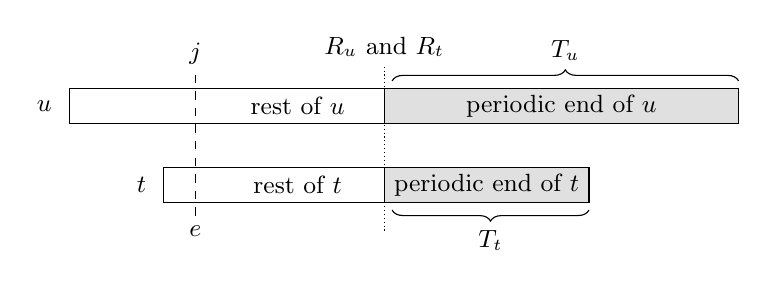
\begin{tikzpicture}[x=1cm,y=1cm,font=\small]
  \draw (1,0.78) rectangle (5,1.22);
  \node at (3.9,1) {rest of $u$};
  \draw[fill=black!12] (5,0.78) rectangle (9.5,1.22);
  \node at (7.25,1) {periodic end of $u$};
  \node[anchor=east] at (0.9,1) {$u$};
  \draw (2.2,-0.22) rectangle (5,0.22);
  \node at (3.9,0) {rest of $t$};
  \draw[fill=black!12] (5,-0.22) rectangle (7.6,0.22);
  \node at (6.3,0) {periodic end of $t$};
  \node[anchor=east] at (2.1,0) {$t$};
  \draw[densely dotted] (5,1.5) -- (5,-0.6);
  \node[above] at (5,1.5) {$R_u$ and $R_t$};
  \draw[dashed] (2.6,1.4) -- (2.6,-0.4);
  \node[above] at (2.6,1.4) {$j$};
  \node[below] at (2.6,-0.4) {$e$};
  \draw[decorate,decoration={brace,amplitude=4pt}] (5.1,1.32) -- (9.5,1.32)
    node[midway,above=4pt] {$T_u$};
  \draw[decorate,decoration={brace,amplitude=4pt,mirror}] (5.1,-0.32) -- (7.6,-0.32)
    node[midway,below=4pt] {$T_t$};
\end{tikzpicture}
\Description{Two horizontal bars, the spine u above the target t. Each bar
consists of an unshaded rest followed by a shaded periodic end. The bars are
placed so that the two boundaries between rest and periodic end lie on one
dotted vertical line. A dashed vertical line through both rests marks a rest
cut j of u and its partner e of t. Braces mark the lengths T_u and T_t of
the two periodic ends.}
\caption{The rest and the periodic end of the spine and of the target for a
purely periodic $\xi$ with least period $\varpi$, drawn with the two boundaries
$R_u$ and $R_t$ on the dotted line. Two cuts in the periodic ends have
equal $\xi$-suffixes if and only if their end distances agree modulo $\varpi$. A
rest cut $j$ of $u$ has an equal $\xi$-suffix with a cut $e$ of $t$ only if $e$ is a rest
cut at the same distance before the boundary, $R_u-j=R_t-e$ (dashed), and
a rest cut never matches a cut of a periodic end (\cref{lem:nm-ends}).}
\label{fig:nm-ends}
\end{figure}

\emph{Deletions.} Delete a factor $w$ from $u=xwy$ and a factor $w'$ from
$t=x'w'y'$, at least one of them nonempty, such that each automaton is in the
same state at both ends of each deleted factor. Then the states at the
remaining cuts are unchanged, so safety, rejection and the endpoint $A(u)$ are
kept. The shortened pair is again a pre-hole that is survivor-free for $\xi$,
provided some head event of $(u,t)$ survives the deletion and every
$\xi$-matched pair of the shortened words comes from a $\xi$-matched pair of the
original words (\cref{lem:nm-deletion}). Two mechanisms provide this lifting.
A factor of the periodic end of $u$ whose length is a multiple of $\varpi$ is
\emph{absorbed}: $w\,(y\xi)=y\xi$, so inserting it back changes no infinite
suffix. \emph{Rigidity}, the non-self-similarity of the suffix after a rest
cut, handles two specific configurations: the synchronous deletion of the
factor between two partnered rest cuts of $u$ together with the factor between
their partners, and the deletion of a factor that ends at an unpartnered rest
cut (\cref{lem:nm-dischargers,lem:nm-four}). A factor that merely ends at a rest
cut can create new matches: for $\xi=0^\omega$, $u=1010$ and $t=110$, deleting
the factor $\wsub u12=0$, which ends at the rest cut $2$, turns $u$ into $t$
and creates the matched pair $(0,0)$. Four deletions, listed in
\cref{tab:nm-deletions}, are found by pigeonhole on the states at the ends of
the factors, the end distance modulo $\varpi$, and one bit recording whether a
head event lies beyond the cut. Write $N_1,\dots,N_4$ for their signature counts
and $C_u$, $U_u$ and $U_t$ for the sets of partnered rest cuts of $u$,
unpartnered rest cuts of $u$, and unpartnered rest cuts of $t$.

\begin{table}[t]
\caption{The four deletions of the pump (\cref{lem:nm-four}). Each applies to a
pre-hole $(u,t)$ for which $\xi$ is survivor-free when the condition in the
second column holds; it deletes the factors in the third column, which are
found by pigeonhole on the signature in the fourth column, of size
$N_i$.}
\label{tab:nm-deletions}
\small
\begin{tabular}{@{}>{\raggedright\arraybackslash}p{1.8cm}>{\raggedright\arraybackslash}p{2.3cm}>{\raggedright\arraybackslash}p{3.3cm}>{\raggedright\arraybackslash}p{2.4cm}l@{}}
\toprule
Deletion & Condition & Deleted factors & Signature & Count\\
\midrule
1, spine end & $T_u\ge T_t+N_1$ & a factor of the periodic end of $u$
  at end distance at least $T_t$ & states of $A$, $A'$; end distance
  mod $\varpi$
  & $N_1=aa'\varpi$\\\addlinespace
2, synchronous rest & $\len{C_u}>N_2$ & the factor between two partnered
  rest cuts of $u$, and the one between their partners & four states, head bit
  & $N_2=2aba'b'$\\\addlinespace
3, spine rest & $\len{U_u}>N_3$ & the factor between two unpartnered rest
  cuts of $u$ & states of $A$, $A'$ & $N_3=aa'$\\\addlinespace
4, target rest & $\len{U_t}>N_4$ & the factor between two unpartnered rest
  cuts of $t$ & states of $B$, $B'$ & $N_4=bb'$\\
\bottomrule
\end{tabular}
\end{table}

If no deletion applies, then the rests are short, since partners inject the
partnered rest cuts of $t$ into those of $u$, so that $R_u\le N_2+N_3$
and $R_t\le N_2+N_4$; the periodic end of $t$ is shorter than $b\varpi$;
and $T_u<T_t+N_1$. Hence both words are shorter than
$N_1+N_2+N_3+N_4+b\varpi=2aba'b'+aa'\varpi+b\varpi+aa'+bb'$
(\cref{lem:nm-count}). Induction on $\len u+\len t$ proves the theorem. No
deletion inside the periodic end of $t$ is needed, and in particular no
factors of both periodic ends are deleted together.

\begin{remark}[An automaton instead of the pump]
Informally, one could instead recognize the survivor-free pre-holes of a
periodic lasso by a two-tape automaton that records a set of spine states for
every residue class of end distances modulo the period. Such an automaton
would have exponentially many states, whereas the pump needs no automaton and
gives a polynomial bound.
\end{remark}

\subsection{The Three Cases}\label{sec:nm-three-cases}

\begin{definition}[Mortal hole]\label{def:nm-mortal-hole}
A \emph{mortal hole} of $I$ is a hole $(u,t)$ such that $A(u)$ is mortal and
$\len t-J(t)<N_A$.
\end{definition}

Put
\[
 \Lnm(a,b,a',b')=4\max\bigl(12aba'b',\ \Pcap(a,b,a',b')\bigr)+6a .
\]
Since $a,b,a',b'\ge1$, this is at most $54a^2ba'b'$, a polynomial in the four
state counts (\cref{app:nm-three-cases}).

\begin{theorem}[Three cases]\label{thm:nm-three-cases}
Let $I$ satisfy \textup{(FH)}. Then $I$ has a hole if and only if at least one
of the following holds:
\begin{enumerate}[label=(\arabic*)]
\item some pre-hole $(u_0,t_0)$ has $A(u_0)$ branching;
\item some pre-hole $(u_0,t_0)$ has $A(u_0)$ thin, and some infinite word safe
from $A(u_0)$ is survivor-free for $(u_0,t_0)$;
\item $I$ has a mortal hole.
\end{enumerate}
More precisely, let $(u,t)=(u_0\theta,t_0\theta)$ be a hole decomposed as in
\cref{lem:nm-decomposition}. If $A(u_0)$ is branching, $(u_0,t_0)$ satisfies
\textup{(1)}. If $A(u_0)$ is thin and $A(u)$ is not mortal, then $(u_0,t_0)$
satisfies \textup{(2)} with an infinite word that begins with $\theta$.
Otherwise $(u,t)$ is a mortal hole. Moreover, if \textup{(1)} or \textup{(2)}
holds, then $I$ has a hole $(u,t)$ with $\len u+\len t\le\Lnm(a,b,a',b')$; this
part does not need \textup{(FH)}.
\end{theorem}

A pre-hole as in (1) is shortened by \cref{prop:nm-short-prehole}, keeping its
endpoint, and completed by \cref{lem:nm-breaker}. In case (2) the infinite
word is a lasso $\xi$ of the thin state $q=A(u_0)$ (\cref{lem:nm-thin}(c)). If
$\xi$ is not purely periodic, every pre-hole with endpoint $q$ is
survivor-free for $\xi$ (\cref{lem:nm-aperiodic}), so
\cref{prop:nm-short-prehole} shortens the pre-hole; if $\xi$ is purely
periodic, its least period is at most $N_A$ and the pump shortens it. In both
cases \cref{cor:nm-lasso-completion} completes the short pre-hole. Conversely,
\cref{lem:nm-decomposition} decomposes a hole as $(u_0\theta,t_0\theta)$. If
$A(u_0)$ is branching, case (1) holds. Otherwise, if $A(u_0)$ is thin and
$A(u)$ has an infinite safe continuation $\xi'$, then $\theta\xi'$ is safe from
$A(u_0)$ and survivor-free, because its prefix $\theta$ already breaks every
obligation. In the remaining cases $A(u)$ is mortal, and
\cref{lem:nm-thin}(a) and~(d) give $\len t-J(t)=\len\theta<N_A$. The proofs are
in \cref{app:nm-three-cases}.

\begin{corollary}[Short holes outside the mortal case]\label{cor:nm-short-holes}
Let $I$ satisfy \textup{(FH)}. Then $I$ has a hole if and only if it has a
hole $(u,t)$ with $\len u+\len t\le\Lnm(a,b,a',b')$ or it has a mortal hole.
\end{corollary}

\begin{proof}
A hole of either kind is a hole. Conversely, if $I$ has a hole, then by
\cref{thm:nm-three-cases} one of (1)--(3) holds; in cases (1) and (2) the theorem
provides a hole with $\len u+\len t\le\Lnm(a,b,a',b')$.
\end{proof}

The bound $\Lnm$ depends on neither the alphabet nor the self guard. The
alphabet enters only the number of candidate pairs, and the self guard is
absorbed by the use of $\max(\len{u_0},\len{t_0})$ in
\cref{lem:nm-breaker,cor:nm-lasso-completion} and by the pump, whose
signatures already contain the states of $B$.

\begin{remark}[When mortal holes cannot occur]\label{rem:nm-nonblocking}
Informally, if no state reachable from $0$ in $\mathcal G_A$ is mortal, for
example if $\Bad=\varnothing$ and $\len\Sigma\ge1$, then case (3) does not
arise, and only the short holes of \cref{cor:nm-short-holes} matter.
\end{remark}

\begin{example}[Condition (FH) is needed]\label{ex:nm-fh}
Let $\Sigma=\{\ell\}$, let $A$, $A'$ and $B$ have the single state $0$, with
$\Bad=\varnothing$, $\Rej=\{0\}$ and $\Guard=\GuardS=\varnothing$, let $B'$ have
the states $0$ and $1$, with $B'(0,\ell)=B'(1,\ell)=1$, and let
$\Head=\{(0,1)\}$. The pair $(\eps,\ell)$ is a hole, with the head event
$(0,1)$, but $I$ has no pre-hole: every target has $J(t)=0$, so a pre-hole has
$t_0=\eps$, whose only aligned pair $(\len{u_0},0)$ carries the state $0$ of
$B'$. Since the only state of $A$ is thin, none of the cases (1)--(3) holds.
Condition (FH) fails: the head $\gamma=\ell$ has $B'(\gamma)=1$, and its proper
prefix $\eps$ is rejected.
\end{example}
